\documentclass{article}

% VARIABLES
\title{ESQUEMA DEL INFORME}
\author{INTEGRANTES}
\date{\today}

% Paquetes para codificación y lenguaje
\usepackage[utf8]{inputenc}                            % Codificación
\usepackage[english, spanish]{babel}                   % Lenguaje
\usepackage{csquotes}                                  % COmpatibilidad con BibLatex
\spanishdecimal{.}                                     % Punto decimal

% Paquetes para matemáticas
\usepackage{amsmath, amsthm, amssymb}                  % Matemáticas
\usepackage{mathptmx}

% Paquetes para geometría y diseño de página
\usepackage[margin=2.5cm, headheight=2cm]{geometry}    % Márgenes

% Paquetes para gráficos y figuras
\usepackage{graphicx}                                  % Imágenes
\usepackage{wrapfig}                                   % Figuras a la derecha

% Paquetes para hipervínculos
\usepackage{hyperref}                                  % Hipervínculos
\hypersetup{
    colorlinks=true,
    linkcolor=black,
    urlcolor=blue,
    citecolor=blue,
}

% Paquetes para encabezados y pies de página
\usepackage{fancyhdr}
\pagestyle{fancy}

% Encabezado y pie de página
\rhead{\title}
\lhead{}
\cfoot{}
\rfoot{\thepage}

% Paquetes adicionales
\usepackage{caption}
\usepackage{xcolor}                                    % Colores personalizados
	\definecolor{codegreen}{rgb}{0,0.5,0}
	\definecolor{codegray}{rgb}{0.5,0.5,0.5}
	\definecolor{codepurple}{rgb}{0.5,0,0.5}
	\definecolor{backcolour}{rgb}{0.95,0.95,0.95}
\usepackage{listings}                                  % Para código
\usepackage[backend=biber,style=apa]{biblatex}         % Bibliografía
\addbibresource{referencias.bib}


% Otras configuraciones
\setlength{\parindent}{0pt}                               % Indentación
\setlength{\parskip}{7pt}                                  % Espaciado entre párrafos
\renewcommand{\baselinestretch}{1.5}                       % Interlineado
\addto\captionsspanish{\renewcommand{\tablename}{Tabla}}   % Redefinir el nombre de la tabla
\addto\captionsspanish{\renewcommand{\figurename}{Figura}} % Redefinir el nombre de la tabla

% Definir el estilo para el código
\lstdefinestyle{CodeStyle}{
    backgroundcolor=\color{backcolour},
    commentstyle=\color{codegreen},
    keywordstyle=\color{codepurple},
    numberstyle=\tiny\color{codegray},
    stringstyle=\color{codepurple},
    basicstyle=\ttfamily\footnotesize,
    breakatwhitespace=false,
    breaklines=true,
    captionpos=b,
    keepspaces=true,
    numbers=left,
    numbersep=5pt,
    showspaces=false,
    showstringspaces=false,
    showtabs=false,
    tabsize=2
}

\begin{document}
\maketitle
\newpage


%HAY QUE RESUMIR ALGUNAS COSAS, COMO LAS INVESTIGACIONES PREVIAS, DEJAR SOLO LO MAS IMPORTANTE%
\section{INDICE}
[implementar indice]
\newpage
\section{INTRODUCCION}
[aca iria la introduccion]
\section{OBJETIVOS}
[Breve descripcion de lo que fue solicitado como proyecto]
\section{PLANIFICACION DEL PROYECTO}
[describir paso a paso que se buscaba hacer, ideas descartadas, por que fueorn descartadas, cual era nuestro objetivo de un usuario, tanto en interfaz como experiencia dentro de loopweb]
\section{LOOP WEB}
['vender' loopweb]
\section{INVESTIGACIONES PREVIAS}
[aca iria la investigacion sobre las redes sociales y la investigacion sobre algoritmos de similitud]
\subsection{{\textbf{Analisis de las redes sociales}}}
El proyecto \textbf{LoopWeb}
trata sobre la creacion de una \textbf{red social}, previamente se necesita realizar una investigacion extensiva sobre las distintas redes sociales que existen actualmente, 
principalmente se necesita saber que hace que \textbf{Bluesky} sea tan especial como para ser el referente maximo para este proyecto.

\section{{\textbf{Bluesky}}}
Es una plataforma de redes sociales descentralizada que se fundó como una iniciativa de investigación como parte de Twitter en 2019. 
Inicialmente, el sitio era solo por invitacion, pero se abrio al publico en febrero.
En otras palabras \textbf{Bluesky} se podria denominar como el nuevo \textbf{Twitter}.

\subsection*{¿Que lo diferencia de otras redes sociales?}
\textbf{Bluesky} es especial porque combina las ventajas de la descentralizacion (propiedad de datos, flexibiidad, diversidad de comunidades)
con la facilidad de uso de las plataformas centralizadas, ofreciendo a los usuarios un control nunca antes visto sobre sus cuenta.
''Bluesky es una red social abierta que ofrece a los creadores independencia de las plataformas, a los desarrolladores libertad de creación y a los usuarios la posibilidad de elegir su experiencia'', afirma la plataforma en su página social.
\begin{itemize}
    \item \textbf{Caracteristicas}
    \begin{itemize}
        \item Feed algorítmico:
        Permite a sus usuarios personalizar el contenido que desean ver, es un tipo de visualizacion de contenido en el que las publicaciones se ordenan segun la relevancia y el interes para el usuario, en lugar de la cronologia.
        \item Moderacion del contenido:
        Cuenta con multiples opciones para que los usuarios puedan sentirse comodos utilizando esta red social. Desde silenciar hashtags y palabras hasta bloqueo de cuentas.
        \item Limite de caracteres:
        Los post son mas cortos, cuenta con un limite de 300 caracteres, y pueden incluir fotos y videos.
    \end{itemize}    
    \item \textbf{Funcionalidades}:
        Permite a los usuarios compartir mensajes breves, interactuar con otros, consumir contenido y participar en conversaciones globales.
    \item \textbf{Algoritmo}:
        Su característica más disruptiva son los feeds personalizados, que permiten a los usuarios construir su propia experiencia algorítmica.
        La magia de Bluesky reside en la posibilidad de gestionar feeds especificos basados en intereses, palabras clave o listas de usuario, lo cual se gestiona en el buscador de la red social.
\end{itemize}
\subsection*{¿Que podriamos sacar de Bluesky?}
A nivel personal creo que uno de los puntos mas fuertes de Bluesky es el feed, ya que permite tener una experiencia mas personalizada al navegar por la red social,
siempre aparecera el contenido que mas le guste al usuatrio, evitando ver post que generen disgusto.
Se puede crear un propio feed que permite un mejor viaje a travez de la red social, eligiendo distintos contenidos para visualizar, no como otras redes sociales que basan el algoritmo en base a likes e interacciones. 

\section{{\textbf{Spotify}}}
Spotify es una plataforma de musica, podcasts y videos digitales que da acceso a millones de canciones.
\subsection*{¿Como funcionan las recomendaciones?}
Los creadores de esta red social saben que no hay dos oyentes iguales, por lo que la experiencia para cada usuario y muchas de las recomendaciones, son personalizadas.
Algunas recomendaciones se basan en la seleccion editorial, como una playlist de musica creada por editores musicales.Otras recomendaciones se adaptan al gusto unico de cada oyente, como una playlist personalizada.
\begin{itemize}
    \item Seleccion editorial:
    Los editores utilizan datos estadisticos y una comprension de las tendencias culturales para ubicar el contenido donde tiene mas probabilidades de ser relevante.
    \item Recomendaciones personalizadas:
    A medida que el usuario interactua en spotify, ya sea con acciones como buscar, escuchar, saltar o guardar en la biblioteca influye en la interpretacion de los gustos.A esto se le llama "perfil de gustos" lo cual da al algorito una indicacion de lo que le gusta al usuario.
    \item Informacion compartida:
    Las recomendaciones tambien se basan en la ubicacion(no precisa) del usuario, idioma, edad, seguidos.
\end{itemize}

\section{{\textbf{Facebook}}}
Facebook es la principal red social que existe en el mundo. Una red de vínculos virtuales, cuyo principal objetivo es dar un soporte para producir y compartir contenidos. 
\subsection*{¿Como recomienda amigos?}
Las sugerencias de amistad se basan en factores como:
\begin{itemize}
    \item Amigos en comun.
    \item Ciudad, escuela, trabajo.
    \item Pertenecer a un mismo grupo en Facebook.
    \item Etiquetas en publicaciones, fotos.
    \item Contactos telefonicos vinculados.
\end{itemize}

\section{{\textbf{X}}}
X es un servicio que permite que los grupos de amigos, familiares y compañeros de trabajo se comuniquen y estén en contacto a través de mensajes rápidos y frecuentes.
\subsection*{¿Como funciona el algoritmo?}
X basa sus recomendaciones en:
\begin{itemize}
    \item Repost(publicaciones compartidas).
    \item Respuestas(comentarios).
    \item Suscripcion:
        Los usuarios que poseen una suscripcion activa aparecen mas en el feed recomendado.
    \item Tendencias:
        Para garantizar que la red social sea la mejor forma de conocer las ultimas noticias y novedades.
    \item Likes en publicaciones.
\end{itemize}

\section{{\textbf{Youtube}}}
Es un sitio web dedicado a compartir videos, presenta una variedad de clips, programas de television, videos musicales, gameplays, videoblogs.
\subsection*{¿Como funcionan sus recomendaciones?}
\begin{itemize}
    \item Encuestas:
    Se envían millones de encuestas al mes (aunque es probable que a un mismo usuario solo le salgan dos o tres) para pedir opiniones sobre los vídeos de la plataforma.
    \item Intereses:
    Se tiene en cuenta cuándo los usuarios hacen clic en "No me interesa" en los vídeos.
    \item Interacciones:
    Se tiene en cuenta el número de likes, dislikes y las veces que se ha compartido un vídeo.
\end{itemize}

\section{{\textbf{TikTok}}}
TikTok permite crear, editar y subir vídeos propios o de terceros inicialmente con una duración máxima de un minuto a los que se les incluyen fondos musicales o sonidos.
\subsection*{¿Como funciona el algoritmo de TikTok?}
El algoritmo de TikTok es una fórmula patentada que determina qué videos de TikTok se muestran a cada usuario.Los principales factores que influyen en el algoritmo de TikTok son las interacciones de los usuarios, la información de los videos y la configuración del dispositivo y la cuenta.
\begin{itemize}
    \item Interacciones del usuario:
        \begin{itemize}
            \item Likes, comentarios, favoritos, seguidos.
            \item Videos marcados como no me interesa.
            \item Videos denunciados.
        \end{itemize}
    \item Informacion de videos:
        \begin{itemize}
            \item Sonidos, efectos.
            \item Hashtags, temas de actualidad.
        \end{itemize}
    \item Configuracion del dispositivo y de la cuenta:
        \begin{itemize}
            \item Preferencia linguistica.
            \item Configuracion del pais.
            \item Tipo de dispositivo movil.
        \end{itemize}
\end{itemize}
   
\section{{\textbf{Instagram}}}
Instagram es una red social principalmente visual, donde un usuario puede publicar fotos, videos e historias de corta duracion.
\subsection*{Algoritmo de Instagram}
No hay un solo algoritmo que decide lo que se ve, ya que cada parte de la app (el feed, la sección "Explorar" y los Reels) tiene su propio sistema de clasificación según cómo es usado.
\begin{itemize}
    \item Contenido de la publicacion:
    El algoritmo tiene en cuenta el tipo de contenido, como fotos, videos o historias, asi como hashtags utilizados.
    \item Recomendaciones personalizadas:
    El sistema se basa en el comportamiento promedio del usuario. Analiza de forma automatizada interacciones como likes, comentarios y publicaciones guardadas. 
    Por lo tanto, las cuentas con las que más interactúa serán priorizadas en su feed. 
\end{itemize}
Actualmente, el algoritmo de Instagram da prioridad a las publicaciones más recientes.

\section{{\textbf{¿Que podemos aplicar de estas redes en el proyecto LoopWeb?}}}
Muchas de estas redes sociales tienen algoritmos, caracteristicas importantes, por lo tanto se deberian aplicar en \textbf{LoopWeb}, principalmente son:
\begin{itemize}
    \item Feed personalizado de Bluesky\\
        Es muy importante la opcion que ofrece esta red social, en la que el usuario puede personalizar el feed a su gusto, ya que entrega una navegacion mas amigable con cada usuario.
    \item Personas que quizas conozcas de Facebook e Instagram\\
        Al tener una red social es muy importante las recomendaciones de amigos que se le hacen al usuario.Y esto es algo que Facebook logra satisfactoriamente, ya que enfoca sus recomendaciones en amigos de amigos, edad, ciudad, grupos, lo cual 
        aumenta la posibilidad de que la sugerencia de amistad pueda ser del agrado del usuario.
    \item Limite de caracteres de Bluesky y X\\
        Tener un limite de caracteres es necesario para que no se haga tediosa la navegacion por la red social.
    \item Bloquear, eliminar y agregar usuarios\\
        Tanto agregar como bloquear y eliminar usuarios es algo fundamental en una red social, para poder mantener el circulo de amigos limpio.
\end{itemize}

\section{{\textbf{Teoria de los grafos en analisis de redes sociales}}}
Imagina las redes sociales como una gigante telaraña donde cada usuarios representa un punto de conexión. 
La teoría de grafos nos ayuda a entender esta telaraña ¿Cómo? Representando cada usuario como un punto (o nodo) y cada conexión entre usuarios como una línea (o arista). 
Esto nos permite ver quién está conectado con quién y cómo interactúan en la red.\\
La teoria de los grafos permite relacionar usuarios que comparten gustos, intereses.
\subsection*{Grafos aplicados a redes sociales}
Cuando hablamos de grafos aplicados a redes sociales lo más común es que se usen para “detectar comunidades”. 
Gracias a los algoritmos podemos ver características, atributos y relaciones que coinciden dentro de un grupo. 
Cuando se analizan los subgrafos, 
podremos ver lo vértices que están más relacionados entre sí, y además cómo se relacionan con el resto de vértices.

\section{BUSQUEDA DE EFICIENCIA}
[investigacion de implementacion de json en c,investigacion sobre bubblesort a mergesort]
\subsection*{Algoritmos de ordenamiento}
Los \textbf{algoritmos de ordenación} son un conjunto de instrucciones que toman un arreglo o lista como entrada y organizan los elementos en un orden particular.
Las ordenaciones suelen ser numéricas o una forma de orden alfabético (o lexicográfico), y pueden ser en orden ascendente (AZ, 0-9) o descendente (ZA, 9-0).

\subsection*{¿Por que son importantes?}
Dado que a menudo pueden reducir la complejidad de un problema, los \textbf{algoritmos de ordenación} son muy importantes en informática. 
Estos algoritmos tienen aplicaciones directas en algoritmos de búsqueda, algoritmos de bases de datos, algoritmos de estructura de datos y muchos más.

\subsection*{Algunos algoritmos de ordenacion} 
\begin{enumerate}
    \item  \textbf{Selection sort}:
    Selection Sort o Ordenamiento por Selección, busca el elemento más pequeño en el conjunto de elementos y lo coloca en la posición correcta. 
    Luego, busca el siguiente elemento más pequeño y lo coloca en la siguiente posición correcta. Repite este proceso hasta que todos los elementos estén ordenados.
    \begin{figure}[H]
        \centering % Para que aparezca centrada
        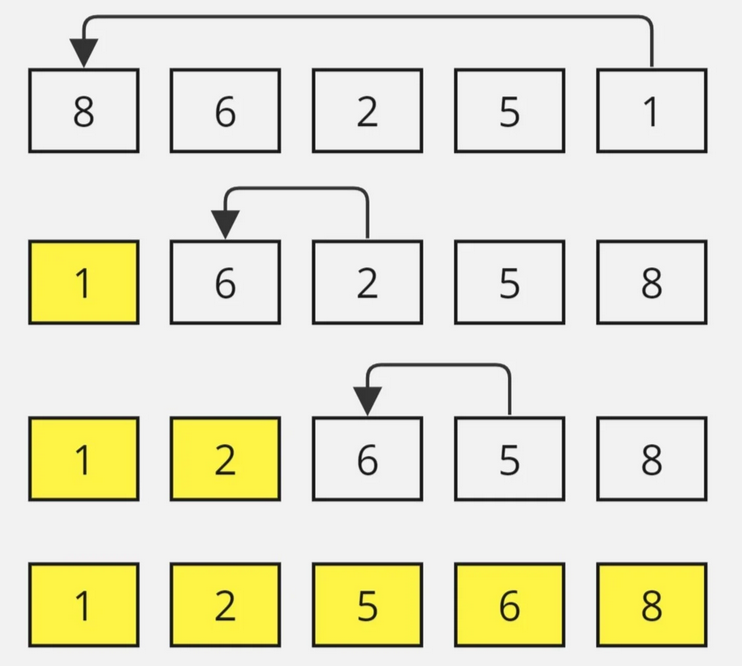
\includegraphics[width=0.5\textwidth]{./src/images/selectionSort.png} % Esta linea incluye la imagen
        \caption{Selection Sort} % Este es el mensaje que acompaña la imagen
        \label{fig:imagen 1} % Esta es la referencia a la imagen
    \end{figure}
    \newpage

    \item \textbf{Bubble sort}:
    Bubble sort o Ordenamiento de Burbuja, compara pares de elementos adyacentes y los intercambia si están en el orden incorrecto. 
    Repite este proceso hasta que todos los elementos estén ordenados.
    \begin{figure}[H]
        \centering % Para que aparezca centrada
        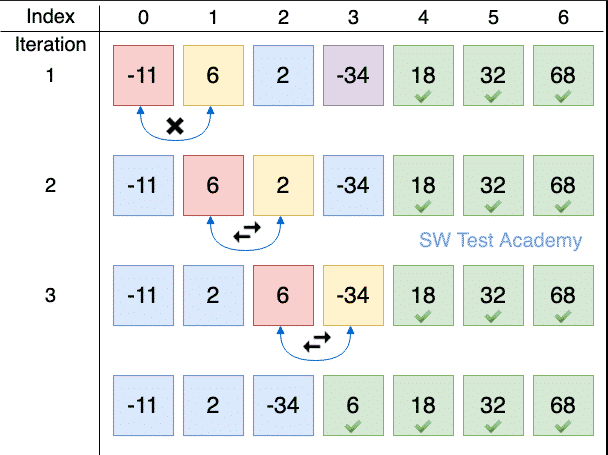
\includegraphics[width=0.5\textwidth]{./src/images/BubbleSort.png} % Esta linea incluye la imagen
        \caption{Bubble Sort} % Este es el mensaje que acompaña la imagen
        \label{fig:imagen 2} % Esta es la referencia a la imagen
    \end{figure}
    

    \item \textbf{Insertion sort}:
    Insertion Sort o Ordenamiento por Inserción, divide el conjunto de elementos en una parte ordenada y otra desordenada. 
    Toma un elemento de la parte desordenada y lo inserta en la posición correcta en la parte ordenada. Repite este proceso hasta que todos los elementos estén ordenados.
    \begin{figure}[H]
        \centering % Para que aparezca centrada
        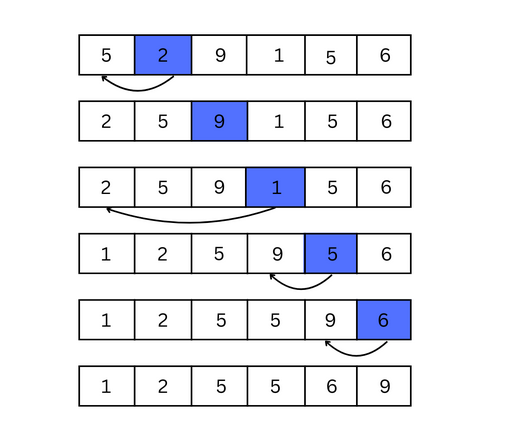
\includegraphics[width=0.5\textwidth]{./src/images/InsertionSort.png} % Esta linea incluye la imagen
        \caption{Insertion Sort} % Este es el mensaje que acompaña la imagen
        \label{fig:imagen 3} % Esta es la referencia a la imagen
    \end{figure}
    \newpage

    \item \textbf{Merge sort}:
    Merge Sort o Ordenamiento por Mezcla, divide el conjunto de elementos en subconjuntos más pequeños, 
    los ordena por separado y luego los fusiona para obtener un conjunto ordenado más grande. 
    Este algoritmo utiliza una estrategia de divide y vencerás.
    \begin{figure}[H]
        \centering % Para que aparezca centrada
        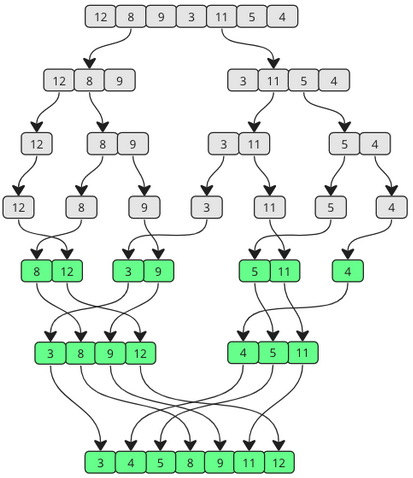
\includegraphics[width=0.5\textwidth]{./src/images/MergeSort.png} % Esta linea incluye la imagen
        \caption{Merge Sort} % Este es el mensaje que acompaña la imagen
        \label{fig:imagen 4} % Esta es la referencia a la imagen
    \end{figure}

    \item \textbf{Heap sort}:
    Heap Sort o Ordenamiento por Montículos, construye un montículo a partir de los elementos y luego extrae sucesivamente el elemento máximo (o mínimo) del montículo, 
    reajustando el montículo después de cada extracción. 
    El resultado final es un conjunto de elementos ordenados.
    \begin{figure}[H]
        \centering % Para que aparezca centrada
        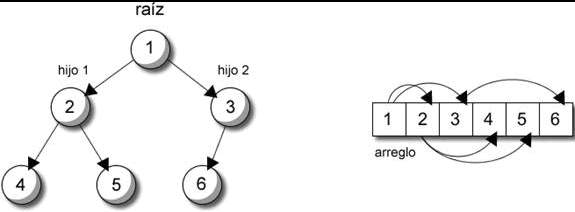
\includegraphics[width=0.5\textwidth]{./src/images/HeapSort.png} % Esta linea incluye la imagen
        \caption{Heap Sort} % Este es el mensaje que acompaña la imagen
        \label{fig:imagen 5} % Esta es la referencia a la imagen
    \end{figure}
    \newpage

    \item \textbf{Quick sort}:
    Quick Sort o Ordenamiento Rápido, elige un elemento llamado "pivote" y divide el conjunto en dos subconjuntos, 
    uno con elementos menores que el pivote y otro con elementos mayores. 
    Luego, aplica el mismo proceso de forma recursiva en cada uno de los subconjuntos. Este algoritmo también utiliza la estrategia de divide y vencerás.
    \begin{figure}[H]
        \centering % Para que aparezca centrada
        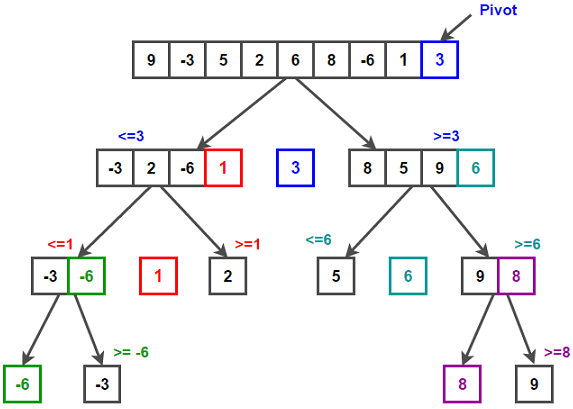
\includegraphics[width=0.5\textwidth]{./src/images/QuickSort.png} % Esta linea incluye la imagen
        \caption{Quick Sort} % Este es el mensaje que acompaña la imagen
        \label{fig:imagen 6} % Esta es la referencia a la imagen
    \end{figure}
    \end{enumerate}
%APLICACION DE JSON EN C%
\section{JSON}
\textbf{JSON} sus siglas en inglés son por JavaScript Object Notation. 
Se trata de un formato para guardar e intercambiar información que cualquier persona pueda leer. 
Los archivos json contienen solo texto y usan la extensión .json.

\subsection*{¿Para qué se utiliza un archivo JSON?} % Esto sería un subtítulo
\textbf{JSON} es un formato que almacena información estructurada y se utiliza principalmente para transferir datos entre un servidor y un cliente.
Un archivo json puede contener diversos datos, como se muestra en la \textbf{Figura 1.}

\begin{figure}[H]
    \centering % Para que aparezca centrada
    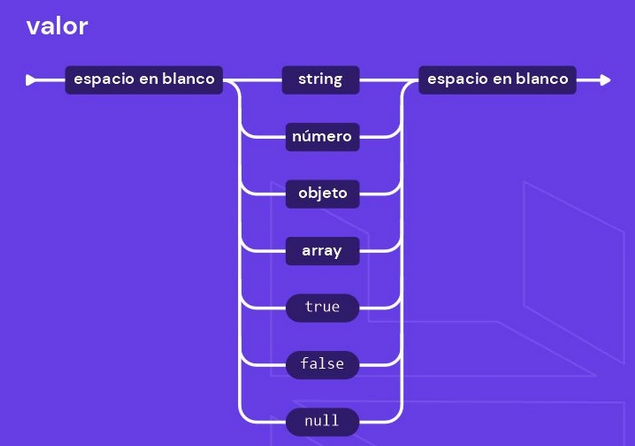
\includegraphics[width=0.5\textwidth]{./src/images/json.png} % Esta linea incluye la imagen
    \caption{Diagrama json} % Este es el mensaje que acompaña la imagen
    \label{fig:imagen} % Esta es la referencia a la imagen
\end{figure}
\textbf{Tipos de datos que se pueden almacenar en JSON:}
\begin{itemize}
    \item Strings: conjunto de caracteres almacenado como objeto.
    \item Numero: se utilizan para datos numericos (edad,peso,etc).
    \item Objeto: estructura de datos que permite almacenar un conjunto de pares clave-valor. Es una manera de organizar y representar datos relacionados entre sí de forma estructurada.
    \item Array:  colección de datos del mismo tipo. Sirve para manejar un número “n” de elementos en común.
    \item Booleanos: valores que son true o false.
    \item  Null: ausencia de un valor o dato.
\end{itemize}
\newpage
\subsection*{Json aplicado en codigo}
\begin{lstlisting}[style=CodeStyle, language=C, caption={Ejemplo de .json}, label={lst:codigo}]
    [
        {
            "nombre": "Juan Perez",
            "curso": "septimo basico",
            "edad":"12",
            "contacto":{
                "correo": "juanperez@gmail.com",
                "movil": "+569 12345678"
            },
            "asignaturas": ["matematicas","lenguaje","fisica"],
            "asistencia":false,
            "deportes":NULL
        }
    ]
\end{lstlisting}
Este .json contiene informacion sobre un objeto, en este caso es un estudiante, el cual almacena: nombre, curso, edad, contacto, asignaturas cursadas, asistencia diaria, deportes a los cuales asiste.
Tambien se podria utilizar un archivo .txt, pero tiene algunas desventajas ante un archivo json.\\\\
\textbf{Ventajas de utilizar un archivo json}
    \begin{itemize}
        \item Estructura bien definida: json tiene una estructura estandar, basada en  objetos y arreglos.
        \item Compatibilidad universal: ampliamente utilizado, soportado en la mayoria de lenguajes de programacion.
        \item Facil de entender y modificar: existen muchas bibliotecas que permiten leer y escribir json.
    \end{itemize}
    \textbf{Desventajas de utilizar un archivo de texto}
    \begin{itemize}
        \item  Falta de estructuras: es un archivo de texto plano.
        \item  Sin soporte directo para datos complejos: no puede manejar directamente  arreglos, booleanos, etc.
        \item  Mas propenso a errores: al no tener una estructura definida es mas probable cometer errores al guardar, agregar o eliminar datos.
    \end{itemize}

\newpage

\subsection*{¿Como utilizar json en \textbf{c}?}
Al estar trabajando en lenguaje c, no es posible aplicar directamente archivos .json, por lo tanto se debe
encontrar la forma de poder leer .json en c. 
Para hacer esta tarea posible existen librerias externas las cuales se deben instalar, algunas de estas son:
\begin{enumerate}
    \item Jansson
    \item Json-c
    \item cjson
\end{enumerate}
En este caso se trabajara con la libreria Jansson.

\section{Libreria Jansson}
Jansson es una libreria de C para decodificar y manipular datos JSON.Se caracteriza por ser simple e intuitivo, 
sin dependencias de otras librerias y posee una documentacion completa.

\subsection*{Funciones de Jansson}
Posee diversas funciones, en este caso no se utilizaran todas. Las funciones mas importantes que se utilizaran en este codigo son:
\begin{enumerate}
    \item  \textbf{json\_error\_t}: 'declara' una especie de 'variable' que almacena informacion sobre cualquier error de analisis que pudiese ocurrir al leer el archivo JSON, necesario al trabajar con json\_loadf y otras funciones.
    \begin{lstlisting}[style=CodeStyle, language=C, caption={json\_error\_t}, label={lst:codigo}]
        json_error_t error;
    \end{lstlisting}
    \item  \textbf{json\_t}: se utiliza para 'declarar' un json, siempre a travez de un puntero.
    \begin{lstlisting}[style=CodeStyle, language=C, caption={json\_t}, label={lst:codigo}]
                json_t *materias_json = json_object_get(alumnos_json,"materias");
    \end{lstlisting}
    \item  \textbf{json\_loadf(FILE *input, unsigned flags, size\_t *flags\_out);}: encargada de cargar el contenido del archivo JSON en una 'variable' del tipo json\_t. Pide tres parametros:
    \begin{itemize}
        \item FILE *imput: archivo .json que se utilizara.
        \item unsigned flags: banderas con las que cuenta la libreria jansson.
        \item size\_t *flags\_out: puntero a una variable (puede ser NULL)
    \end{itemize}
    \begin{lstlisting}[style=CodeStyle, language=C, caption={json\_loadf}, label={lst:codigo}]
        json_t *json = json_loadf(archivo,0,&error);
    \end{lstlisting}
    \item  \textbf{json\_object\_get(json\_t *obj, const char *key)}: se utiliza para acceder a los valores de un objeto json, sus parametros son:
    \begin{itemize}
        \item json\_t *obj:  puntero a un objeto json.
        \item const char *key: dato que se quiere obtener, por ejemplo 'nombre'.
    \end{itemize}
    \begin{lstlisting}[style=CodeStyle, language=C, caption={json\_object\_get}, label={lst:codigo}]
        json_object_value(alumnos_json,"nombre");
    \end{lstlisting}
    \item  \textbf{json\_string\_value(json\_t *json)}: extrae el valor de una cadena de texto, necesita un unico parametro (de donde se quiere obtener el string).
    \begin{lstlisting}[style=CodeStyle, language=C, caption={json\_string\_value}, label={lst:codigo}]
        json_string_value(json_object_value(alumnos_json,"nombre");)
    \end{lstlisting}
    En este caso se esta obteniendo la cadena de texto 'nombre' que se encuentra en el json alumnos.
    \item  \textbf{json\_interger\_value(json\_t *json)}: obtiene el valor de un dato de tipo entero, solo pide un unico parametro (de donde se quiere obtener el string).
    \begin{lstlisting}[style=CodeStyle, language=C, caption={json\_interger\_value}, label={lst:codigo}]
        json_interger_value(json_object_value(alumnos_json,"edad");)
    \end{lstlisting}
    En este caso se esta obteniendo el entero 'edad' que se encuentra en el json alumnos.
\end{enumerate}

\section{¿Como aplica esto en loopweb?}
Los algoritmos de ordenacion son de suma importancia, actualmente se esta utilizando \textbf{bubble sort}, pero  este algoritmo es conocido por ser lento e ineficiente en la mayoria de los casos,
especialmente cuando se enfrenta a conjunto de datos grandes, por lo tanto en este caso no es recomendable utilizarlo, pero hay otro algoritmo que si puede ser muy efectivo,
este algoritmo es \textbf{merge sort} el cual es de los mas eficientes algoritmos de busqueda y ordenamiento, es a menudo la mejor opción para ordenar una lista enlazada.

\subsection*{Referencia merge sort en codigo}
\begin{lstlisting}[style=CodeStyle, language=C, caption={merge()}, label={lst:codigo}]
    void merge(int arr[], int l, int m, int r) {
        int i, j, k;
        int n1 = m - l + 1; ///< Numero de elementos en el subarreglo izquierdo.
        int n2 = r - m; ///< Numero de elementos en el subarreglo derecho.
        int L[n1], R[n2]; ///< Subarreglos izquierdo y derecho.
        
        for (i = 0; i < n1; i++){
            L[i] = arr[l + i]; ///< Copia de datos al subarreglo izquierdo.
        }
        for (j = 0; j < n2; j++){
            R[j] = arr[m + 1 + j]; ///< Copia de datos al subarreglo derecho.
        }
        i = 0; ///< Indice para el subarreglo izquierdo L.
        j = 0; ///< Indice para el subarreglo derecho R.
        k = l; ///< Indice para el arreglo original arr.
    
        // Fusion de los subarreglos 
        while (i < n1 && j < n2) {
            if (L[i] <= R[j]) {
                arr[k] = L[i]; ///< Toma el elemento de L si es menor o igual que el de R.
                i++;
            } else {
                arr[k] = R[j]; ///< Toma el elemento de R si es menor que el de L.
                j++;
            }
            k++;
        }
        // Copia los elementos restantes de L si los hay
        while (i < n1) {
            arr[k] = L[i]; ///< Copia el elemento de L al arreglo original.
            i++;
            k++;
        }
        // Copia los elementos restantes de R si los hay
        while (j < n2) {
            arr[k] = R[j]; ///< Copia el elemento de R al arreglo original.
            j++;
            k++;
        }
    }
\end{lstlisting}

\section{ESTRUCUTURAS DE DATOS IMPLEMENTADAS}
[¿Por que decidimos implementar estas estructuras de datos y no otra?]
\section{ALGORITMOS DE ORDENAMIENTO}
 ¿Por que implementamos cierto algotirmo de ordenamiento y no otro?
\section{FUNCIONAMIENTO DE LOOPWEB}
[aca iria algo asi como, comentarios, amigos, etc, explicar un poco como funciona]

%COMENTARIOS%
\subsection*{Comments}
Para la lectura de datos de \textbf{LoopWeb} se utilizaron las listas enlazadas para ir guardando de comentario en comentario del archivo 
en el que se lee(importante saber que la separacion de los comentarios es con una linea blanca entera)
en el cual tambien se incluyen los tags de \textbf{GenreLikes} y \textbf{BandLikes} los cuales se guardan por comentario
y van guardando su cantidad como el tag en si mismo 
\subsection*{curiosidades de codigo} 
A continuación se hace una mencion de curiosidades del codigo:
\begin{enumerate}
    \item Isalnum(): es una funcion que devuelve true si el caracter es alfanumerico, esta funcion se utilizo en un proyecto anterior para crear la tokenizacion del indice invertido
    \item Creacion de comentarios: la funcion \textbf{appendComments} crea un nodo de comentarios y en este se guardan los tags de géneros y bandas
    \item Tags: son guardados en arreglos de char de tamaño \textbf{MAXTAGS} y cada uno de ellos tiene un tamaño de \textbf{MAXTAGLENGTH}
\end{enumerate}

\section{FUNCIONES IMPLEMENTADAS}
Breve descripcion de funciones implementadas mas extracto de codigo

%FUNCION getOTP, falta agregar extracto de codigo%
\subsection*{Funcion GetOTP}
\textbf{getOTP} es una funcion que recibe como argumento un string de texto y devuelve un entero que representa
el código de acceso al cual queremos entrar. Para esto se utiliza un bucle while que tiene como condición que el caracter
que estamos leyendo sea un número distinto a -1 ya que este seria un caracter que no corresponde con un código de acceso.\\
Principalmente la funcion es \textbf{getOTP()} pero esta funcion solo se puede usar para condiciones de una palabra, Como por ejemplo
\textbf{./main.o -a,./main.o -u} pero no \textbf{./main.o --administrador} o \textbf{./main.o --user}. ya que estas opciones son muy largas para la funcion
por lo cual si utilizamos la funcion \textbf{getoptLong()} podemos ocupar las opciones \textbf{./main.o -a},\textbf{./main.o -u} y \textbf{./main.o --administrador},\textbf{./main.o --user}
\subsection*{Importante saber para implementar \textbf{getoptLong}}
\begin{enumerate}
    \item Hacer un archivo \textbf{getotp.h} prototipo de esta función dado de esta manera: int getoptlong(int argc, char * const argv[],const char *optstring,const struct option *longopts,int *longindex);
    \item \textbf{Struct option}, este struct se encarga de almacenar toda la información necesaria para poder usar la funcion \textbf{getoptLong()}.
    \item Dentro del main: hacer el struct option y definir cuales son las opciones a usar y si requieren argumento o no.
    \item Al utilizar \textbf{./main.o -administrador} tener en cuenta que tiene que ser doble guión, sino puede causar problemas, pero si se quiere utilizar \textbf{./main.o --a} no hay problemas dado que tambien lo toma como administrador, al igual que si se deja la palabra incompleta, por ejemplo \textbf{./main.o --admi}
\end{enumerate}

%FUNCION MERGESORT%
\subsection*{Implementacion de mergeSort\_genreLinkList}
\begin{lstlisting}[style=CodeStyle, language=C, caption={split\_genreLinkList}, label={lst:codigo}]
    /**
    * @brief Divide una lista enlazada en dos mitades.
    *
    * @param source Puntero al nodo inicial de la lista a dividir.
    * @param frontRef Referencia a la primera mitad de la lista.
    * @param backRef Referencia a la segunda mitad de la lista.
    */
   void split_genreLinkList(GenreLinkPosition source, GenreLinkPosition* frontRef, GenreLinkPosition* backRef) {
       GenreLinkPosition slow, fast;
       slow = source;
       fast = source->next;
   
       while (fast != NULL) {
           fast = fast->next;
           if (fast != NULL) {
               slow = slow->next;
               fast = fast->next;
           }
       }
   
       *frontRef = source;
       *backRef = slow->next;
       slow->next = NULL;
   }
\end{lstlisting}

\begin{lstlisting}[style=CodeStyle, language=C, caption={fusion de listas}, label={lst:codigo}]
    /**
 * @brief Fusiona dos listas enlazadas ordenadas en una sola lista ordenada
 *
 * @param a Puntero a la primera lista ordenada
 * @param b Puntero a la segunda lista ordenada
 * @return Puntero al nodo inicial de la lista fusionada ordenada
 */
GenreLinkPosition merge_genreLinkLists(GenreLinkPosition a, GenreLinkPosition b) {
    if (a == NULL) return b;
    if (b == NULL) return a;

    GenreLinkPosition result;

    if (strcmp(a->genre, b->genre) <= 0) {
        result = a;
        result->next = merge_genreLinkLists(a->next, b);
    } else {
        result = b;
        result->next = merge_genreLinkLists(a, b->next);
    }
    return result;
}
\end{lstlisting}

\begin{lstlisting}[style=CodeStyle, language=C, caption={mergerSort\_genreLinkList}, label={lst:codigo}]
    /**
    * @brief Ordena una lista enlazada utilizando el algoritmo merge sort.
    *
    * @param headRef Referencia al puntero del nodo inicial de la lista a ordenar.
    */
   void mergeSort_genreLinkList(GenreLinkPosition* headRef) {
       GenreLinkPosition head = *headRef;
       GenreLinkPosition a, b;
   
       if ((head == NULL) || (head->next == NULL)) {
           return;  /**<si la lista esta vacia o tiene un solo elemento, no hay que ordenar */ 
       }
   
       split_genreLinkList(head, &a, &b);
   
       mergeSort_genreLinkList(&a);  /**<ordena la primera mitad */
       mergeSort_genreLinkList(&b);  /**<ordena la segunda mitad */
   
       *headRef = merge_genreLinkLists(a, b);  /**<fusiona las dos mitades ordenadas */
    }
\end{lstlisting}
%JSON EN C%
\section*{Codigo para poder abrir un archivo .json en c}
\begin{lstlisting}[style=CodeStyle, language=C, caption={read\_list\_json}, label={lst:codigo}]
    /**
 * @brief Funcion para leer un arreglo de strings .json y almacenarlos en una matriz
 * 
 * @param array_json  objeto json del tipo arreglo  que contiene los valores se van a leer
 * @param matriz  donde se acumularan los valores leidos del arreglo
 * @return cantidad de elementos leidos
 */
int read_list_json(json_t *array_json, char matriz[MAX_ELEMENTS][MAX_CADENA]) {
    size_t cantidad = json_array_size(array_json);/**<obtener el numero de elementos en el arreglo json*/
    if (cantidad > MAX_ELEMENTS) {/**< verificar que no supere la cantidad permitida*/
        printf("max elementos superado\n");
        cantidad = MAX_ELEMENTS;
    }

    for (size_t i = 0; i < cantidad; i++) {
        const char *valor = json_string_value(json_array_get(array_json, i));  /**< obtener el valor del string en el indice i de la matriz*/
        if (!valor) {
            printf("Elemento no valido en indice %zu.\n", i);
            return 0;
        }
        snprintf(matriz[i], MAX_CADENA, "%s", valor); /**<copia el valor del string donde corresponda en la matriz */
    }
    return (int)cantidad; 
}
\end{lstlisting}

\begin{lstlisting}[style=CodeStyle, language=C, caption={read\_archive\_json}, label={lst:codigo}]
    /**
 * @brief Funcion para leer el archivo json, en este caso usuarios.json
 * 
 * @param nombre_archivo  archivo .json a leer
 * @param usuarios  usuario de la estructura antes creada en el que se guardaran los datos obtenidos
 * @param total_users  puntero a un entero en el que se guardara el numero total de usuarios leidos en el .json
 * @return int 
 */
int read_archive_json(const char *nombre_archivo, User usuarios[], int *total_users) {
    FILE *archivo = fopen(nombre_archivo, "r");  /**< Abre el archivo .json en modo lectura */
    if (!archivo) {
        perror("No se pudo abrir el archivo JSON");
        return 1;
    }
    json_error_t error;     /**< declaracion de "variable" error basada en una funcion de la libreria jansson */
    json_t *json = json_loadf(archivo, 0, &error); /**<  puntero en el cual se guarda el archivo .json*/
    fclose(archivo);

    if (!json) {
        printf("Error al analizar el .json: %s\n", error.text);
        return 1;
    }

    *total_users = (int)json_array_size(json);  /**<  tamano total de usuarios basado en el arreglo json, utilizando una funcion de la libreria jansson*/
    for (int i = 0; i < *total_users; i++) {
        json_t *usuario_json = json_array_get(json, i); /**< Obtiene el objeto json, basada en el usuario[i] */

        /**<  Lectura de campos basicos*/
        const char *name = json_string_value(json_object_get(usuario_json, "nombre"));  /**<  almacena el nombre del usuario[i]*/
        json_int_t age = json_integer_value(json_object_get(usuario_json, "edad"));     /**<  almacena la edad del usuario[i]*/
        const char *nationality = json_string_value(json_object_get(usuario_json, "nacionalidad"));  /**< almacena la nacionalidad del usuario[i] */
        json_t *gustos_json = json_object_get(usuario_json, "gustos");  /**< almacena los gustos del usuario[i] */
        json_t *bands_json = json_object_get(usuario_json, "bandas");   /**< almacena las bandas del usuario[i] */
        json_t *friends_json = json_object_get(usuario_json, "amigos"); /**< almacena los amigos del usuario[i] */

        snprintf(usuarios[i].name, sizeof(usuarios[i].name), "%s", name);  /**<  copia el nombre a la estructura user*/
        usuarios[i].age = (int)age;                                        /**<  copia la edad a la estructura user*/
        snprintf(usuarios[i].nationality, sizeof(usuarios[i].nationality), "%s", nationality);   /**< copia la nacionalidad a la estructura user */

       /**< Lee y almacena las listas de gustos, bandas, amigos en la estructura user */
        read_list_json(gustos_json, usuarios[i].gustos);
        read_list_json(bands_json, usuarios[i].bands);
        read_list_json(friends_json, usuarios[i].friends);
    }

    json_decref(json); /**< libera la memoria utilizada por el json, funcion de la libreria jansson */
    return 0;
}
\end{lstlisting}

\begin{lstlisting}[style=CodeStyle, language=C, caption={main.c}, label={lst:codigo}]
#include <stdio.h>
#include "funciones.h"

int main() {
    User usuarios[MAX_USERS];
    int total_users = 0;

    if (read_archive_json("usuarios.json", usuarios, &total_users) == 0) {
        printf("Se leyeron %d usuarios:\n", total_users);

        /**<  imprimir los datos obtenidos de cada usuario*/
        for (int i = 0; i < total_users; i++) {
            printf("ID %d:\n", i + 1);
            printf("Nombre: %s\n", usuarios[i].name);
            printf("Edad: %d\n", usuarios[i].age);
            printf("Nacionalidad: %s\n", usuarios[i].nationality);
            printf("Gustos:\n");
            for (int j = 0; j < MAX_ELEMENTS && usuarios[i].gustos[j][0]; j++) {
                printf("  - %s\n", usuarios[i].gustos[j]);
            }
            printf("Bandas:\n");
            for (int j = 0; j < MAX_ELEMENTS && usuarios[i].bands[j][0]; j++) {
                printf("  - %s\n", usuarios[i].bands[j]);
            }
            printf("Amigos:\n");
            for (int j = 0; j < MAX_ELEMENTS && usuarios[i].friends[j][0]; j++) {
                printf(" ID - %s\n", usuarios[i].friends[j]);
            }
            printf("\n");
        }
    }
    return 0;
}

\end{lstlisting}

\section{APARIENCIA DE LOOPWEB}
[aca irian las primeras ideas de como se veria un perfil y de finalmente como se muestra(creo que esa parte la hizo rodolfo)]


\section{CONCLUSION}

\newpage

\nocite{*}
\printbibliography[heading=bibintoc]

\end{document}